\chapter[Princípios de Automação Residencial]{Princípios básicos de um sistema
de automação residencial e monitoramento energético}
\label{chap:principios}
%Note que, como o nome do capítulo é muito longo, fornecemos um nome abreviado para uso no cabeçalho

Este capítulo apresenta uma visão abrangente dos princípios fundamentais na concepção, implementação e operação de um sistema inteligente de automação residencial orientado ao monitoramento e previsão do consumo energético. O contexto abordado parte da realidade de residências convencionais, isto é, aquelas que não dispõem de infraestrutura prévia de automação, exigindo assim soluções flexíveis, escaláveis e capazes de integrar múltiplos dispositivos e tecnologias. Nosso enfoque não se limita ao simples acionamento de equipamentos, mas abrange a coleta e análise detalhada de dados, permitindo uma gestão mais eficiente dos recursos, redução de custos, melhoria do conforto e incremento da sustentabilidade ambiental.

Iniciamos com um exame minucioso da arquitetura típica de um sistema de automação residencial, descrevendo os principais componentes: sensores (ambientais, de presença, de consumo energético), atuadores (termostatos, dimmers, motores para cortinas, entre outros), controladores (centralizados e distribuídos), protocolos de comunicação (Wi-Fi, Zigbee, Z-Wave, BLE, Thread e \textit{Matter}) e interfaces de usuário (aplicativos, painéis físicos, assistentes de voz). Destacamos, em especial, o \textit{Matter}, um protocolo emergente que unifica e facilita a interoperabilidade entre dispositivos de diferentes fabricantes, garantindo flexibilidade, segurança e escalabilidade ao ecossistema doméstico conectado.

Em seguida, detalhamos o processo de instrumentação do sistema, abordando a seleção criteriosa de hardware, a integração de sensores e atuadores, bem como a definição da topologia da rede. Esse cuidado assegura a qualidade dos dados coletados, a robustez do controle e a adequação às normas legais. A segurança da informação e a privacidade são tratadas de forma transversal, observando-se os princípios da Lei Geral de Proteção de Dados (LGPD) e adotando medidas como criptografia, autenticação de dispositivos, minimização de dados e consentimento informado dos usuários.

Outro ponto central é o monitoramento energético. Não se trata apenas de registrar o consumo, mas de transformar dados brutos em conhecimento. São exploradas técnicas de pré-processamento, análise estatística, aprendizado de máquina e Controle Estatístico de Processo (CEP) para detectar anomalias, identificar padrões de consumo, antecipar demandas e propor intervenções que otimizem o uso de energia. Essas abordagens analíticas embasam decisões proativas, possibilitando desde ajustes automáticos de cargas elétricas até a recomendação de substituição de equipamentos ineficientes, o que resulta em benefícios econômicos, maior conforto e redução do impacto ambiental.

Ao compreender as soluções existentes, suas limitações e potenciais, este capítulo fornece uma base sólida para os desenvolvimentos subsequentes, orientando tanto a implementação prática do protótipo quanto a evolução do sistema no sentido de maior inteligência, integração e respeito à privacidade e às leis vigentes.

\section{Arquitetura de um Sistema de Automação Residencial}

A arquitetura de um sistema de automação residencial é composta por diversos elementos que trabalham em conjunto para oferecer controle, monitoramento e otimização de aspectos como eficiência energética, segurança, conforto e conveniência. Ela não consiste apenas em dispositivos isolados, mas em um ecossistema integrado capaz de entender as condições do ambiente, agir de forma proativa e se adaptar às preferências dos moradores.

A seguir, detalhamos os principais elementos dessa arquitetura, estabelecendo as bases para compreender as complexidades e potencialidades de tais sistemas.

\subsection{Sensores}

Os sensores representam a interface entre o mundo físico e o digital. Eles coletam dados sobre o ambiente e o estado dos dispositivos, fornecendo informações essenciais para que o sistema possa tomar decisões informadas. Podem monitorar temperatura, umidade, luminosidade, qualidade do ar, presença de pessoas e consumo de energia, entre outros parâmetros. Alguns exemplos:

\begin{itemize}
    \item \textbf{Sensores de movimento e presença}: Utilizam tecnologias como infravermelho passivo (PIR), ultrassom ou micro-ondas. Além de acionar luzes ou alarmes, podem colaborar na climatização, ajustando a temperatura apenas em ambientes ocupados.
    \item \textbf{Sensores ambientais (temperatura, umidade, qualidade do ar)}: Auxiliam no controle de sistemas de HVAC (Aquecimento, Ventilação e Ar Condicionado), garantindo conforto térmico e qualidade do ar interno.
    \item \textbf{Sensores de luminosidade}: Ajustam iluminação artificial conforme a luz natural, otimizando o uso de energia e melhorando o bem-estar.
    \item \textbf{Sensores de consumo energético}: Medem o consumo de dispositivos específicos ou circuitos, fornecendo dados granulares para análise, detecção de aparelhos ineficientes e implementação de estratégias de economia de energia.
\end{itemize}

A seleção e instalação adequadas dos sensores são fundamentais, influenciando a qualidade dos dados coletados e a efetividade das estratégias de controle.

\subsection{Atuadores}

Atuadores transformam as decisões do sistema em ações físicas. Podem ser relés, motores, dimmers ou válvulas controladas eletronicamente, acionando iluminação, climatização, cortinas, persianas, eletrodomésticos e outros dispositivos.

\begin{itemize}
    \item \textbf{Interruptores e dimmers inteligentes}: Ligam, desligam ou ajustam a intensidade luminosa, criando cenários adequados para diferentes atividades.
    \item \textbf{Termostatos inteligentes}: Regulam o aquecimento ou resfriamento, aprendendo rotinas e antecipando demandas, reduzindo custos e melhorando o conforto.
    \item \textbf{Motores para cortinas e persianas}: Controlam entrada de luz e calor, integrando-se a sensores de luminosidade e temperatura para otimizar a eficiência energética.
    \item \textbf{Tomadas inteligentes}: Permitem ligar e desligar aparelhos remotamente, fornecendo dados de consumo e contribuindo para reduzir o uso excessivo de energia.
\end{itemize}

A qualidade, confiabilidade e responsividade dos atuadores são essenciais para garantir que as decisões do sistema sejam efetivamente postas em prática.

\subsection{Controladores}

Os controladores são o “cérebro” do sistema, processando as informações dos sensores e enviando comandos aos atuadores. Podem ser centralizados ou distribuídos, e sua complexidade varia desde microcontroladores simples até sistemas embarcados sofisticados e servidores locais.

\begin{itemize}
    \item \textbf{Controlador Centralizado}: Uma unidade concentra a lógica, facilitando a manutenção, porém criando um ponto único de falha.
    \item \textbf{Controladores Distribuídos}: Cada área ou cômodo pode ter seu próprio controlador, tornando o sistema mais robusto e escalável.
    \item \textbf{Inteligência Artificial e Aprendizado de Máquina}: Permitem o ajuste dinâmico dos parâmetros de controle com base em dados históricos, antecipação de demandas e identificação de padrões complexos.
\end{itemize}

A escolha do controlador depende do nível de inteligência desejado, da escalabilidade necessária e da capacidade de processar algoritmos avançados de previsão e otimização.

\subsection{Protocolos de Comunicação}

A comunicação é fundamental para a interação entre sensores, atuadores, controladores e serviços externos. Diversos protocolos existem, cada um com características próprias de alcance, consumo, taxa de dados e segurança.

\subsubsection{Wi-Fi}

Baseado nos padrões IEEE 802.11, é amplamente utilizado por sua disponibilidade em roteadores domésticos, oferecendo alta largura de banda e facilidade de integração. Porém, com muitos dispositivos conectados, pode haver congestionamento e consumo elevado de energia.

\subsubsection{Zigbee}

Baseado no IEEE 802.15.4, foi concebido para baixo consumo de energia e baixa taxa de dados. Adota topologia em malha, ampliando a cobertura da rede. É popular em iluminação e sensores simples, porém a interoperabilidade entre diferentes marcas nem sempre é garantida.

\subsubsection{Z-Wave}

Protocolo proprietário focado em automação residencial, com baixo consumo de energia, topologia em malha e operação em frequências sub-GHz, reduzindo interferências. Oferece boa confiabilidade, embora a dependência da Z-Wave Alliance e sua natureza proprietária limitem a flexibilidade.

\subsubsection{Bluetooth Low Energy (BLE)}

Voltado para baixo consumo de energia e distâncias curtas, é ideal para dispositivos alimentados por bateria e integração com smartphones. Frequente em fechaduras inteligentes, sensores portáteis e dispositivos de rastreamento.

\subsubsection{Thread}

Protocolo baseado em IPv6, permite comunicação direta com a internet, redes em malha e baixo consumo de energia. Facilita a integração de dispositivos em grande escala e é frequentemente associado ao \textit{Matter}.

\subsubsection{Protocolos Proprietários}

Muitos fabricantes têm seus próprios protocolos, geralmente otimizados para funções específicas. Embora possam oferecer certa vantagem inicial, sua interoperabilidade limitada e dependência de fornecedor prejudicam a escalabilidade a longo prazo.

\subsubsection{Matter}

O \textit{Matter} representa uma tentativa da indústria de unificar e padronizar a comunicação entre dispositivos. Desenvolvido pela Connectivity Standards Alliance (CSA) e apoiado por empresas como Apple, Amazon, Google e Samsung, o \textit{Matter} baseia-se em IP e integra transportes como Wi-Fi, Thread e Ethernet.

Seus principais objetivos incluem:

\begin{itemize}
    \item \textbf{Interoperabilidade Universal}: Evitar a necessidade de múltiplos \textit{hubs} ou \textit{bridges}.
    \item \textbf{Segurança Robusta}: Criptografia ponta a ponta, autenticação de dispositivos e certificados operacionais.
    \item \textbf{Facilidade de Configuração}: Utiliza BLE e QR Codes para simplificar o provisionamento.
    \item \textbf{Escalabilidade e Flexibilidade}: Suporta diversas arquiteturas de rede e categorias de dispositivos.
\end{itemize}

\begin{figure}[thpb]
  \centering
  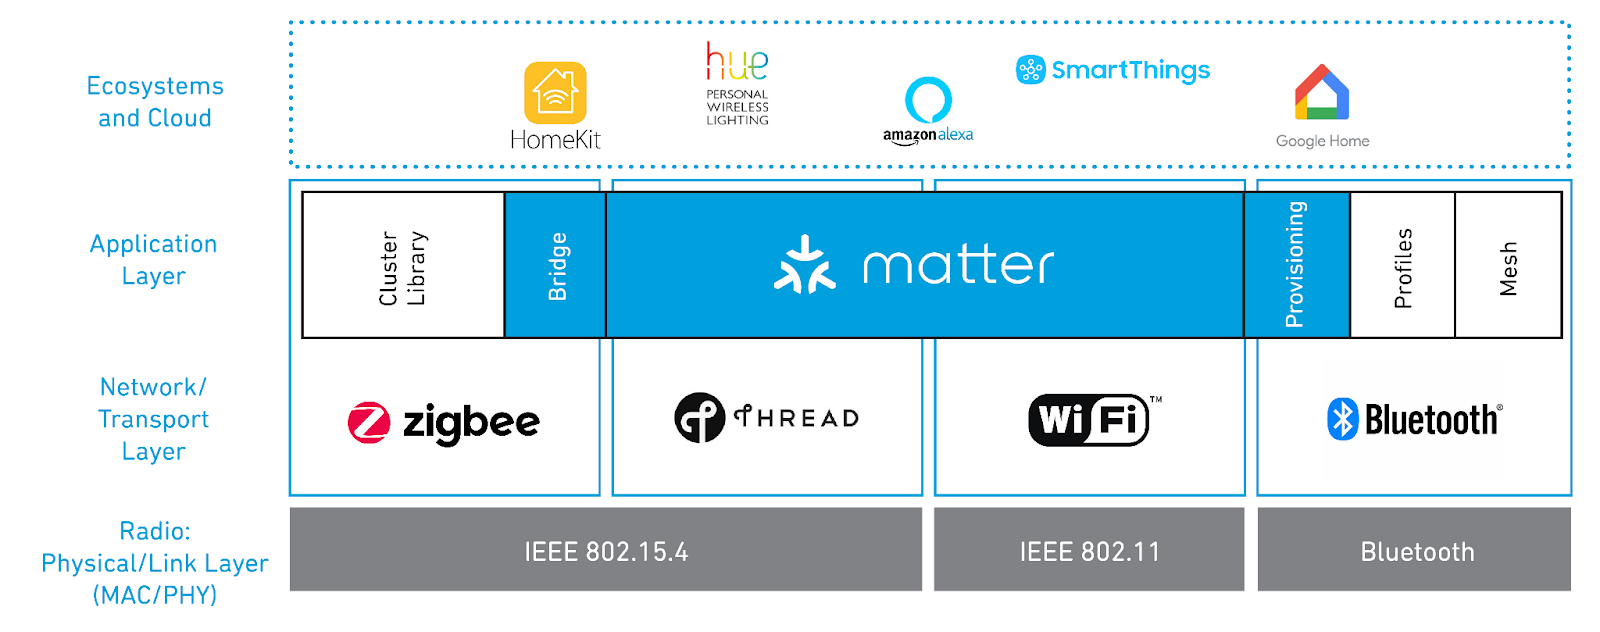
\includegraphics[width=0.9\textwidth]{DescricaoProcesso/Figuras/matter_big_arc.png}
  \caption{Arquitetura do \textit{Matter} como camada de aplicação.}
  \label{fig:matter-layer}
\end{figure}

Como descrito em \cite{matter_spec}, o protocolo Matter garante interoperabilidade entre diferentes dispositivos.

\subsection{Interface de Usuário}

A interface de usuário conecta pessoas e sistema, permitindo controle e monitoramento:

\begin{itemize}
    \item \textbf{Aplicativos Móveis e Web}: Acesso em qualquer lugar, visualização de histórico, criação de cenários e recebimento de notificações.
    \item \textbf{Painéis Físicos}: Telas sensíveis ao toque instaladas nas paredes, facilitando ajustes rápidos.
    \item \textbf{Assistentes Virtuais de Voz}: Google Assistant, Alexa, Siri, oferecendo controle sem a necessidade de interfaces gráficas.
\end{itemize}

Com o \textit{Matter}, a experiência do usuário é aprimorada, pois um único aplicativo ou assistente pode controlar dispositivos de diferentes marcas.

\subsection{Serviços em Nuvem e Análise de Dados}

A nuvem possibilita armazenamento histórico, análise avançada e integração com serviços externos:

\begin{itemize}
    \item \textbf{Análise Preditiva}: Antecipar consumos futuros, otimizar uso de energia.
    \item \textbf{Tarifas Dinâmicas}: Ajustar consumo conforme variação de preços de energia.
    \item \textbf{Manutenção Preditiva}: Identificar falhas iminentes em equipamentos.
\end{itemize}

A nuvem também permite acesso remoto, controle global e integração de APIs de terceiros, ampliando a funcionalidade do sistema.

\subsection{Segurança e Privacidade}

A crescente conectividade na automação residencial traz desafios que vão além de questões técnicas, abrangendo também a proteção de dados e o cumprimento de leis como a Lei Geral de Proteção de Dados (LGPD) no Brasil e o Regulamento Geral sobre a Proteção de Dados (GDPR) na União Europeia. Nesse contexto, é indispensável adotar medidas de segurança cibernética e garantir a privacidade dos moradores, protegendo suas informações pessoais e rotinas. O sistema deve incorporar, desde a fase de projeto, uma abordagem de \textit{Privacy by Design}, assegurando que mecanismos de proteção e conformidade estejam integrados às suas camadas mais básicas.

As principais práticas incluem:

- \textbf{Criptografia}: Todos os dados sensíveis coletados, transmitidos e armazenados devem ser protegidos por criptografia robusta, tornando-os ilegíveis a terceiros não autorizados. Assim, mesmo em caso de interceptação do tráfego de rede, informações pessoais não serão expostas, cumprindo princípios de segurança e confidencialidade exigidos pela LGPD.

- \textbf{Autenticação de Dispositivos}: Garantir que apenas dispositivos autenticados e confiáveis acessem a rede doméstica. Isso envolve a implementação de certificados digitais, chaves criptográficas ou outros métodos de autenticação forte. A restrição de acesso a dispositivos não autorizados previne usos indevidos das informações e atende aos princípios de prevenção e segurança previstos na LGPD.

- \textbf{Atualizações Seguras}: Manter o firmware dos dispositivos atualizado, corrigindo vulnerabilidades e garantindo um nível adequado de segurança contínua. O processo de atualização deve ser autenticado e seguro, impedindo que versões maliciosas sejam instaladas. Essa prática previne incidentes que possam expor dados pessoais e assegura a conformidade com a LGPD, pois reduz o risco de violações de segurança.

A privacidade é igualmente crítica. Dados sobre hábitos e rotinas dos moradores, bem como informações sobre ocupação da residência, uso de dispositivos específicos e preferências pessoais, devem ser armazenados e processados de modo a garantir o respeito à LGPD. Isso significa adotar princípios como minimização da coleta de dados (coletar apenas o indispensável para a finalidade proposta), consentimento informado dos usuários, transparência sobre como e por que os dados são usados e possibilidade de exclusão dos mesmos mediante solicitação. Além disso, todas as práticas de tratamento de dados devem estar documentadas e auditáveis, para comprovação de conformidade quando necessário.

\subsection{Integração com Outros Sistemas}

A automação residencial não funciona isoladamente. Ela pode integrar-se a sistemas de segurança, entretenimento, eletrodomésticos inteligentes e geração distribuída de energia, formando um ecossistema mais rico e funcional. Por exemplo, o sistema pode ajustar o uso de energia com base na produção solar local ou desativar determinados dispositivos ao detectar que a casa está vazia. No entanto, ao integrar múltiplos sistemas e plataformas, a complexidade na gestão dos dados aumenta. Nesse cenário, é fundamental garantir que todos os serviços externos cumpram também as normas de privacidade e segurança, incluindo a LGPD, mantendo assim a coerência e a proteção dos dados em todo o ecossistema.

\subsection{Escalabilidade e Flexibilidade}

A capacidade de crescer e se adaptar às mudanças é vital. Um sistema de automação residencial deve suportar a adição de novos dispositivos, tecnologias e serviços sem exigir reestruturações complexas. O uso de padrões abertos, como o \textit{Matter}, fortalece a escalabilidade e flexibilidade, garantindo que o sistema possa evoluir junto com o usuário e o mercado. Neste contexto, qualquer expansão deve manter o mesmo nível de conformidade com a LGPD, ampliando as práticas de segurança e privacidade para acomodar novos fluxos de dados, dispositivos e funcionalidades sem comprometer a proteção das informações pessoais.

\subsection{Instrumentação do Processo}

A instrumentação do processo envolve a seleção, instalação e configuração de sensores, atuadores e controladores. Esse cuidado na instrumentação não apenas assegura a qualidade dos dados e a efetividade das ações executadas, como também garante que o tratamento das informações coletadas obedeça aos princípios da LGPD e demais normas de proteção de dados. Para isso, alguns cuidados adicionais devem ser tomados:

- \textbf{Seleção de Hardware}: Além de atender às faixas de operação e às especificações técnicas, é importante escolher sensores e atuadores de fabricantes comprometidos com práticas adequadas de segurança e privacidade. O hardware deve permitir a implementação de criptografia, controle de acesso e atualizações seguras. Dispositivos que já seguem padrões abertos e oferecem mecanismos de proteção de dados facilitam a conformidade legal.

- \textbf{Topologia da Rede}: Ao projetar a rede, deve-se garantir cobertura de sinal, minimizar interferências e assegurar redundância em redes \textit{mesh}. Além da confiabilidade técnica, a topologia deve permitir segmentação da rede, isolando dispositivos críticos daqueles com maior risco de vulnerabilidades. Essa separação física ou lógica dificulta acessos não autorizados a dados sensíveis, contribuindo para a privacidade e segurança dos moradores.

- \textbf{Integração Elétrica}: A correta instalação elétrica, observando segurança, aterramento, fusíveis e normas técnicas, assegura não apenas o bom funcionamento dos componentes, mas também evita falhas que possam comprometer a segurança das informações. Curto-circuitos ou picos de tensão inesperados podem afetar módulos de segurança, chaves criptográficas ou até mesmo corromper dados sensíveis.

- \textbf{Provisionamento de Dispositivos}: A configuração inicial dos endereços, chaves de segurança e rotinas de atualização deve ser realizada de forma segura, garantindo que o dispositivo só seja controlado por usuários autorizados. Além disso, políticas de senhas fortes, autenticação de dois fatores e gestão de chaves criptográficas são práticas recomendadas. Essa etapa é essencial para assegurar conformidade com a LGPD, já que uma falha na configuração inicial pode resultar em acesso indevido a dados pessoais, comprometendo a privacidade dos moradores.

Em suma, a instrumentação não é apenas um aspecto técnico; ela é o alicerce para a proteção dos dados, a manutenção da segurança e o respeito à privacidade. Ao combinar boas práticas de engenharia com requisitos legais, o sistema de automação residencial pode operar de forma confiável, eficiente e em total conformidade com a LGPD e outras normas de proteção de dados.

\section{Monitoramento Energético}
\label{sec:monitoramento_energetico}

O monitoramento energético é um elemento central para a compreensão aprofundada do uso de recursos em um ambiente residencial automatizado. Mais do que simplesmente quantificar o consumo de eletricidade, o monitoramento energético permite revelar padrões, prever demandas futuras, identificar ineficiências e propor intervenções corretivas ou preventivas. Ao integrar dados provenientes de diversos sensores — incluindo aqueles dedicados à medição de corrente e tensão em circuitos específicos, bem como às tomadas e equipamentos inteligentes —, o sistema obtém uma visão holística do comportamento energético da residência.

Abaixo, são detalhadas as principais etapas e aspectos relacionados ao monitoramento energético, com especial ênfase na análise de dados, privacidade, conformidade com a LGPD, aplicações práticas e o uso de técnicas de controle estatístico de processo.
\subsection{Coleta e Organização dos Dados}

A primeira etapa do monitoramento energético consiste na coleta sistemática de dados relativos ao consumo de eletricidade em diferentes pontos da residência. Esses dados podem ser obtidos por meio de:

\begin{itemize}
    \item \textbf{Sensores de Consumo em Tempo Real}: Dispositivos que medem corrente e tensão, permitindo o cálculo instantâneo da potência e energia consumidas em circuitos específicos ou em eletrodomésticos individuais.
    \item \textbf{Tomadas e Disjuntores Inteligentes}: Elementos capazes de registrar o uso energético de um aparelho conectado, bem como ligar ou desligar o fornecimento conforme instruções do controlador.
    \item \textbf{Medição Global da Residência}: Sensores posicionados no quadro elétrico principal, fornecendo uma visão macro do consumo, contra a qual se podem comparar dados mais granulares para identificar fontes de ineficiência.
\end{itemize}

A coleta contínua gera um grande volume de dados. Para lidar com isso, é essencial adotar uma infraestrutura de armazenamento e processamento robusta. Uma opção comum é o uso de um \textbf{NAS (Network Attached Storage)}, um dispositivo de armazenamento conectado à rede local que fornece espaço centralizado e seguro para arquivamento dos dados. O NAS permite acesso controlado, backup automático e fácil ampliação da capacidade de armazenamento. Além disso, a utilização de sistemas em nuvem, servidores locais ou híbridos pode complementar o NAS, garantindo resiliência, segurança e acessibilidade dos dados.

Em qualquer cenário, devem-se implementar mecanismos de segurança (criptografia, autenticação forte) e compressão/normalização para facilitar o processamento posterior.

\subsection{Pré-Processamento, Qualidade dos Dados e Controle Estatístico de Processo}

Antes de realizar análises avançadas, os dados coletados precisam passar por etapas de pré-processamento, incluindo:

\begin{itemize}
    \item \textbf{Limpeza de Dados}: Remoção de leituras espúrias, tratamento de valores faltantes e correção de discrepâncias causadas por ruído elétrico ou falhas de comunicação.
    \item \textbf{Agregação e Granularidade}: Ajuste da escala temporal (por exemplo, sumarizar leituras segundo a segundo, minuto a minuto ou hora a hora) e espacial (agrupando dados por cômodo, circuito ou categoria de aparelho).
    \item \textbf{Normalização e Padronização}: Transformação dos dados em escalas comparáveis, permitindo análises consistentes entre diferentes pontos de medição ou períodos.
\end{itemize}

Um conjunto de dados bem pré-processado é mais coerente, confiável e adequado à aplicação de técnicas de análise estatística, aprendizado de máquina e modelagem preditiva.

Nesse contexto, o \textbf{Controle Estatístico de Processo (CEP)} pode ser aplicado ao monitoramento energético como uma ferramenta para acompanhar a variabilidade do consumo ao longo do tempo. Oriundo do domínio da qualidade industrial, o CEP utiliza gráficos de controle e limites estatísticos para distinguir variações normais de anomalias. Aplicado à automação residencial, o CEP permite:

\begin{itemize}
    \item \textbf{Estabelecer Faixas Normais de Operação}: Determinar limites superiores e inferiores para o consumo esperado, considerando padrões históricos e características da residência.
    \item \textbf{Detecção Precoce de Anomalias}: Identificar rapidamente desvios significativos, como um aumento inesperado no consumo de um aparelho, indicando falha ou uso indevido.
    \item \textbf{Monitoramento Contínuo}: Acompanhar a evolução do consumo ao longo do tempo, avaliando se as mudanças implementadas (como troca de um equipamento ou ajuste nas rotinas) resultam em maior eficiência.
\end{itemize}

O CEP atua como um complemento às técnicas de análise mais complexas, ajudando a manter o sistema dentro de parâmetros normais e fornecendo bases para intervenções pontuais.
\subsection{Análise Estatística e Inteligência Artificial}
Com dados limpos e estruturados, bem como limites estatísticos definidos pelo CEP, torna-se possível aplicar uma variedade de técnicas analíticas para extrair valor significativo:

\begin{itemize}
    \item \textbf{Estatística Descritiva}: Cálculo de médias, medianas, desvios-padrão e percentis para caracterizar o perfil de consumo energético ao longo do tempo.
    \item \textbf{Detecção de Anomalias Avançada}: Em conjunto com o CEP, métodos de aprendizado de máquina podem reconhecer padrões não lineares, detectando anomalias sutis que escapariam a métodos estatísticos convencionais.
    \item \textbf{Análise de Correlação e Causalidade}: Estabelecer relações entre o consumo energético e outras variáveis (temperatura, ocupação, eventos externos).
    \item \textbf{Modelagem Preditiva}: Uso de algoritmos de aprendizado supervisionado ou não supervisionado para prever demandas futuras, ajustar parâmetros de controle em tempo real e recomendar intervenções.
    \item \textbf{Clusterização de Perfis de Consumo}: Agrupamento de padrões de uso semelhantes, auxiliando na identificação de zonas energéticas e na otimização personalizada do sistema.
\end{itemize}

A inteligência artificial, combinada ao CEP, amplia as capacidades do sistema, tornando-o mais adaptativo e robusto. Isso resulta em ajustes proativos na operação da residência, reduzindo custos, melhorando o conforto e minimizando impactos ambientais.

\subsection{Privacidade, LGPD e Proteção dos Dados Energéticos}

As informações sobre consumo energético podem revelar hábitos, presença, rotinas e preferências dos moradores. Como tais dados podem ser considerados pessoais ou sensíveis segundo a LGPD, devem ser tratados com o mesmo rigor aplicado a outras informações coletadas:

\begin{itemize}
    \item \textbf{Minimização de Dados}: Coletar apenas o nível de detalhe necessário.  
    \item \textbf{Anonimização e Pseudonimização}: Remover ou mascarar informações identificadoras.
    \item \textbf{Consentimento e Transparência}: Explicar claramente aos moradores como, por que e por quanto tempo os dados serão coletados, analisados e armazenados.
    \item \textbf{Segurança da Informação}: Aplicar criptografia ponta a ponta, autenticação robusta e isolamento de redes.
    \item \textbf{Auditorias e Responsabilização}: Manter registros sobre o tratamento de dados, comprovando conformidade com a LGPD em caso de inspeções.
\end{itemize}

Ao equilibrar análise de dados avançada, CEP e privacidade, o monitoramento energético torna-se não apenas um recurso valioso, mas também uma solução respeitosa aos direitos e expectativas dos usuários.

\subsection{Integração com Outros Sistemas e Evolução Contínua}

O monitoramento energético não existe isoladamente. Ao integrar-se com controladores, sistemas de climatização, iluminação e segurança, bem como com serviços em nuvem e APIs externas, o sistema pode ajustar em tempo real o uso de energia conforme necessidades, demandas e condições externas.

Com a aplicação do CEP, é possível identificar se as integrações e ajustes recomendados estão mantendo o consumo dentro dos limites estatísticos esperados ou se intervenções adicionais são necessárias. Conforme novos dispositivos e tecnologias surgem, a arquitetura flexível e o uso de padrões abertos, como o \textit{Matter}, asseguram que o sistema seja escalável e possa incorporar inovações sem comprometer a segurança, a privacidade ou a qualidade da análise de dados.
\subsection{Benefícios Práticos e Responsabilidade Social}

Quando bem implementado, o monitoramento energético, aliado ao CEP e à análise de dados, traz diversos benefícios:

\begin{itemize}
    \item \textbf{Eficiência e Economia}: Redução de custos com energia elétrica por meio da identificação de desperdícios e ajustes estratégicos.
    \item \textbf{Conforto e Qualidade de Vida}: Ajustes automáticos de parâmetros ambientais conforme preferências e necessidades, sem intervenção manual constante.
    \item \textbf{Sustentabilidade}: Otimização do uso de energia, priorizando fontes renováveis e reduzindo a pegada de carbono.
    \item \textbf{Tomada de Decisão Baseada em Evidências}: Dados claros, validados e dentro de parâmetros estatísticos auxiliares guiam melhorias contínuas e embasadas em fatos.
\end{itemize}

A responsabilidade social emerge ao assegurar que tais benefícios sejam obtidos sem invadir a privacidade ou violar direitos fundamentais. A conformidade com a LGPD, o uso ético da análise de dados e a adoção de CEP garantem que a tecnologia melhore a vida dos moradores, mantendo a confiança e a proteção das informações pessoais.
Em síntese, o monitoramento energético aplicado a um sistema de automação residencial, quando embasado em um arcabouço analítico sólido, conformidade regulatória, uso de CEP e cuidado com a privacidade, transcende a mera coleta de dados. Ele estabelece um processo contínuo de aprendizado, ajuste e otimização que beneficia usuários, meio ambiente e sociedade em geral.  
\bibliography{Monografia}%,library}